\documentclass[letterpaper, 12pt]{article}
\usepackage{cmjStyle}
\usepackage{natbib}
\bibpunct{(}{)}{;}{a}{}{,}
\doublespacing
\raggedright
%\setlength{\parindent}{0} % first para indent?
\setlength{\parskip}{2ex}
\parindent 24pt
\urlstyle{same} % make url tags have the same font
\setcounter{secnumdepth}{-1}

%% The package endfloat moves all floats (figures, tables...) to the
%% end of the paper, as required for the final version of a CMJ paper.
%% Leave this package commented out for initial submission, but
%% uncomment it for final version.
% \usepackage{endfloat}

\begin{document}

%% %author - name
%% {\cmjAuthor Vilson Vieira, Renato Fabbri, Guilherme Lunhani, Geraldo Magela de Castro Rocha Junior}
%% %author - address
%% \newline
%% \begin{cmjAuthorAddress}
%%     Instituto de Física de São Carlos\\
%%     Universidade de São Paulo\\
%%     1234 Anywhere Street\\
%%     Anywhere, Anwhere 012345 USA\\
%%     vilson@void.cc, renato.fabbri@gmail.com, gcravista@gmail.com, gera.sp@gmail.com
%% \end{cmjAuthorAddress}

\vspace*{24pt}

%{\cmjAuthorPhone << AUTHOR TELEPHONE (not for publication): +55 16 8108 7007 >>}

 {\cmjTitle Vivace: A Collaborative Live Coding Language}

% outros títulos.. ??????????
% Vivace: Freak Coding on Your Face

\section*{Abstract}

This paper describes the principles and the design of Vivace, a live
coding language built with Web technologies to be executed, ideally, in
any ordinary browser. It starts by reviewing what motivated and
inspired the creation of the language. That leads to specifications of
the language and how it is parsed and then executed using the recently
created Web Audio API. A brief discussion is then presented on why the Web
is an environment of interest to collaborative live coding and how it
affects the performances. This work concludes by previewing how
Vivace has motivated the creation of ``freak coding'' , a live coding
sub-genre.

\section*{} % Introdução, sem título.

In November of 2011, a live coding trio called \textit{FooBarBaz}
unleashed its first presentation for a wide audience. Its performers
were using two instances of ChucK~\citep*{wang2003chuck} and a
dedicated mixing Puredata + Analog Mixer instance~\footnote{Pictures
  of the presentation available at
  \url{http://www.flickr.com/photos/festivalcontato/6436260557}}. Live
coding has been gaining world wide popularity~\citep*{nilson2007live}, while
remaining quite untouched in Brazil. To the best of our knowledge, that
presentation was the first live coding performance in our
country -- between 3000-5000 attendees were in the
audience where code was used on-the-fly to create the music they were
listening. At same time, two live coding desktop work-spaces were projected
on big screens to the public, following the principles from the
\textsc{toplap} manifesto~\citep*{ward2004live}.

During the performance, the trio used ChucK in an unconventional
way. Instead of writing loops and conditionals, one of the live coders
manipulated parameters of audio files by editing lists of numerical
values together with mnemonic operations like retrograde and
transposition.  The other live coder focused on more fluid lines with
large sounds having evolving characteristics; this contributed with
larger musical arcs.  Audio mixing with Puredata was carried out by the
third performer literally using handwaving gestures tracked by a camera and
our custom-designed color detection algorithms. Live coders used code
templates quick-inserted by programmer text editors (Vi and Emacs). Other visual
resources the performers focused on were: Unix ``cowsay'' generated phrases on
individual terminals and animated bouncing balls -- stimulating the audience to
imitate Rapid Eyes Movements (REM). These artifacts - code, ``cowsay'' phrases,
moving REM-like points of reference, all projected in big screens to the public
-- were incorporated as good practices during the live coding performance.

Therefore, based on those elements, a new language was designed:
Vivace~\footnote{A live demonstration of Vivace is on-line at
  \url{http://vivace.void.cc} ready to be used by everyone using
  Google Chrome or Apple Safari.}~\citep*{Vivace}.  To avoid software
configuration and make it easy to share the session -- and the system
itself -- with everyone, the Web was chosen as the running
environment for Vivace. On every new session performed using Vivace,
new principles were added into the language and, at the same time,
into our artistic behavior.

In summary, this paper is a circle: it describes how performances
motivated the language and how the language itself influenced the
creation of a live coding sub-genre that is being developed by many
hands, called ``freak coding'' by its manifesto~\citep*{freak}, other
written resources, and in spoken instances.

\parskip 18pt

\section{More motivation \& inspiration: arrange the room, the code is dirty}

Vivace is inspired by various live coding languages. The syntax of
Vivace, as shown in Figure~\ref{fig:vivace}, borrows elements from ixi
lang~\citep{magnusson2011ixi} like the use of sequences to control
audio parameters in real time. ABT~\citep{fabbri} and
FIGGUS~\citep{fabbri2} were tightly important to the development of
Vivace as well and we are planning to rewrite some of its components
-- originally in Python -- inside Vivace. ChucK suggested chained unit
generators specified by the $=>$ operator, imitating the object
connections in visual programming languages like Puredata.

\begin{figure}[htpb]
  \begin{center}
    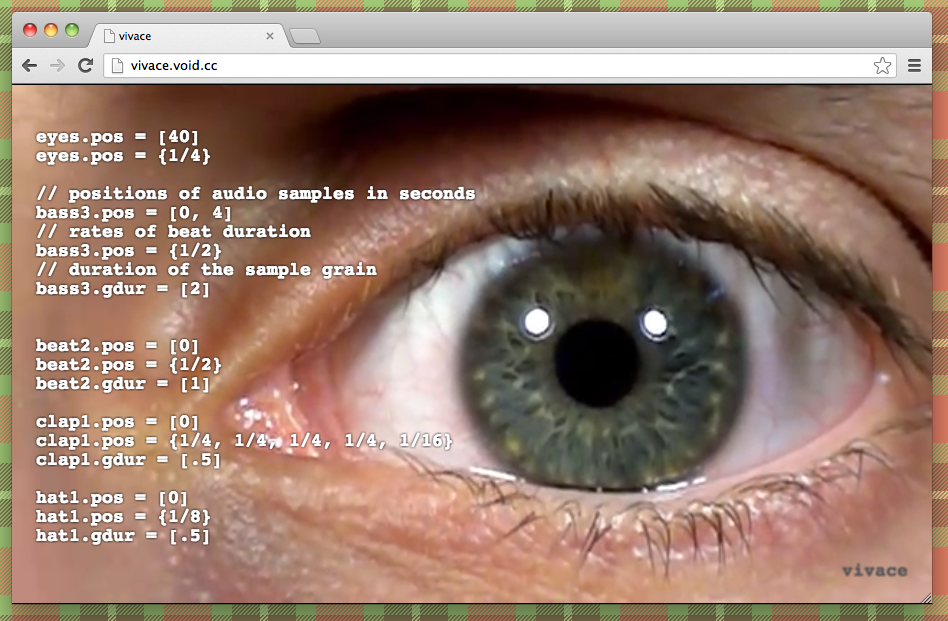
\includegraphics[scale=.3]{img/fig_vivace.png}
    \caption{The Vivace environment.}
    \label{fig:vivace}
  \end{center}
\end{figure}

After the creation of Audio Data API~\citep*{audiodata} and the most
recent Web Audio API~\citep*{webaudio} -- that makes possible to
process audio in real time inside Web browsers -- a collection of
audio Web applications started to emerge. The same is true for live
coding languages and systems.  Thus, along with the \textit{desktop
  languages} pointed above, Vivace was also inspired by Web live
coding languages and is part of this \textit{family} of Web
applications together with Gibber~\citep*{gibber},
livecoder~\citep*{livecoder}, livecoding.io~\citep*{livecodingio} and
livecodelab~\citep*{livecodelab}, to note some of them.

A remarkable difference between Vivace and those languages or
environments is the collaboratively. Vivace was built to make possible
to write code with many hands at the same time, as happens with the
now popular ``pads''~\footnote{Etherpad on:
  \url{http://etherpad.org/}.}, a characteristic easily implemented on
Web.  Another difference is the unconcern to be a Turing-complete
language. This made the design of Vivace more flexible and near to the
music process instead of the computing process (a characteristic
perceived in ixi lang as well). Vivace tries to place itself between
the rigorous of code and the flexibility of artistic expression.

\section{The language (specification) we all speak}

Vivace, as a language~\footnote{The complete language specification
  can be found at
  \url{https://github.com/automata/vivace/wiki/Language-spec}.}, is a
collaborative live coding language with use of extreme simple syntax,
mnemonic operations, easy audio mixing, template editing and audio
parameters automation. The use of shared code, sounds and images leads
to a more complex scenario, thus greater the possibility of
inconsistency of compiled code as well as actions for artistic
result. This enhances the fit of specific language syntax.

Vivace is not an imperative language. Instead of routines and
procedures to control audio attributes, it uses definitions related
with musical scores and the \emph{track paradigm} common on music
production software. It is natural to musicians (and, as we
experienced during performances, also to non-musicians) to understand
a sequence of notes, or audio parameters, repeating over and over
again, than a for-loop and if-chains. In this way, Vivace is a
declarative, domain specific language, based on the following
principles:

\begin{itemize}
  
\item Names are literals like $foo$, $bar$, $baz$ and are defined as
  the user wants.
\item Music is made by voices (instruments).
\item Voices have name, timbre and parameters changing along the time.
\item The language should be simple. ``Freak coders'', with a
  dedicated section below, only define some properties with a set of
  values (i.e. arrays, dictionaries) making it possible to generate
  sequences, even using list comprehension.
\item Mnemonic musical operations (reverse, inverse, transpose) on
  properties by use of syntax sugar: few chars, big results.
\item Timbre are signals made by chains of audio generators and
  filters or video files as described below.
\item Parameters are musical notes, amplitudes, oscillators frequency,
  delay time and so on.
\item Parameters changes their values at specific times and during
  certain durations.

\end{itemize}

Here is a ``Hello, World!'' Vivace code:

\begin{Verbatim}[fontfamily=courier, xleftmargin=\parindent]
 # foo is a simple audio sample, oscillator or video file
 foo.src = youtube('http://www.youtube.com/watch?v=XXX')
 # defining the video positions (in seconds) to be played
 foo.pos = [10, 20, 35]
 # the durations (as time ratios) to play each position
 foo.cdur = [1/2, 1/4, 1/8, 1/16, 1]
\end{Verbatim}

A voice is defined as \textit{foo} and its parameters are specified
using the \textit{dot} operator. Every parameter changes over time as
the values written as numerical sequences, surrounded by brackets. A
special sequence exists to every parameter.  This is all the Vivace
syntax.

There are extra semantics to operate on the sequences. Every sequence
accepts operators: mnemonic commands used to reverse, transpose and
even replace elements of the sequence based on list
comprehensions. Those operations are common in music composition and
having them as mnemonics makes typing fast and handy for live
coding. The next listing presents the standard operators:

\begin{Verbatim}[fontfamily=courier, xleftmargin=\parindent]
# we can use operators
foo.pos = [1, 2, 3] reverse        # result is [3, 2, 1]
foo.pos = [1, 2, 3] inverse        # result is [1, 0, -1]
foo.pos = [1, 2, 3] transpose +2   # result is [3, 4, 5]

# and even list comprehension
foo.pos = [1/i+1 for i in [1, 2, 3]] 
# result is [2, 3, 4]

# or combine both
foo.pos = [1/i+1 for i in [1, 2, 3]] reverse 
# result is [4, 3, 2] as expected
\end{Verbatim}

Vivace is written in JavaScript to take advantage of Web technologies.
To parse Vivace, Jison~\citep*{jison} comes handy, a JavaScript
library that clones Flex and Bison functionality as lexer and
parser. This flexibility to parse and execute new languages as
JavaScript inside every browser opens a remarkable opportunity to
experiment with new syntax and semantics for live
coding. Furthermore, considering the tradition of UI design and
development on Web thanks to HTML and CSS, one can experiment those
new languages with fast prototyped UI -- a requisite already addressed
by live coding languages~\citep*{magnusson2011algorithms} like
Texture~\citep*{mclean2011texture}. Along these advantages, it is
important to note: every live coding language built on Web runs
everywhere a browser is installed. No firewall chain to surpass with
OSC, no software installation and configuration, no dependencies,
people just need to type an URL.

\section{Vivace audio engine}

Before Web Audio API, the only way to create sound in web pages was
using plug-ins. Recently, Web Audio API enabled real time audio
processing on Web browsers~\footnote{At the time this paper was
  written, only Google Chrome and Apple Safari supported the
  API. Mozilla is working to have it running on Firefox as
  well.}. Every routine is written as native code (in C++ and Assembly
when appropriated) to guarantee maximum performance. The API is based
on a convenient and familiar paradigm: audio unit graphs. Web Audio
specifies a collection of nodes (\emph{AudioNode} objects) and
routines to connect and disconnect them. While manipulating those
nodes we can create a large number of audio applications:
synthesizers, filters, analyzers, mixers and even real time audio
engines to live coding. This motivated basic explorations of
multichannel expansion, filtering and audio effects, controlling an
integrated Web audio system.

Every voice in Vivace is represented as a default audio chain such as
the one shown in Figure~\ref{fig:chain}. All audio unit parameters
within this chain (e.g.\ pitch, reverb time, high, medium and low
channel levels, panner values and gain) can be manipulated editing the
code or by sliders on an UI (Figure ~\ref{fig:ui}). This kind of
interface is more familiar to musicians, remembering a real mixer, and
makes possible an adequate treatment of voices timbre and
spacialization of the sound sources by means of parameters like level
of stereophonic channels L and R, quality, central frequency and gain
of a 3-band equalization filter, and reverb time control.

\begin{figure}[htpb]
  \begin{center}
    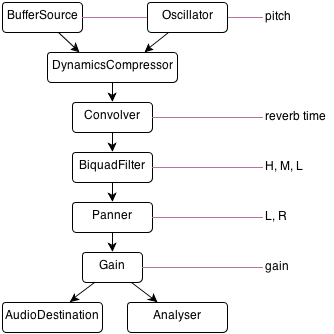
\includegraphics[scale=.5]{img/fig_chain.png}
    \caption{Standard audio unit chains as Web Audio API objects for
      each Vivace voice.}
    \label{fig:chain}
  \end{center}
\end{figure}

\begin{figure}[htpb]
  \begin{center}
    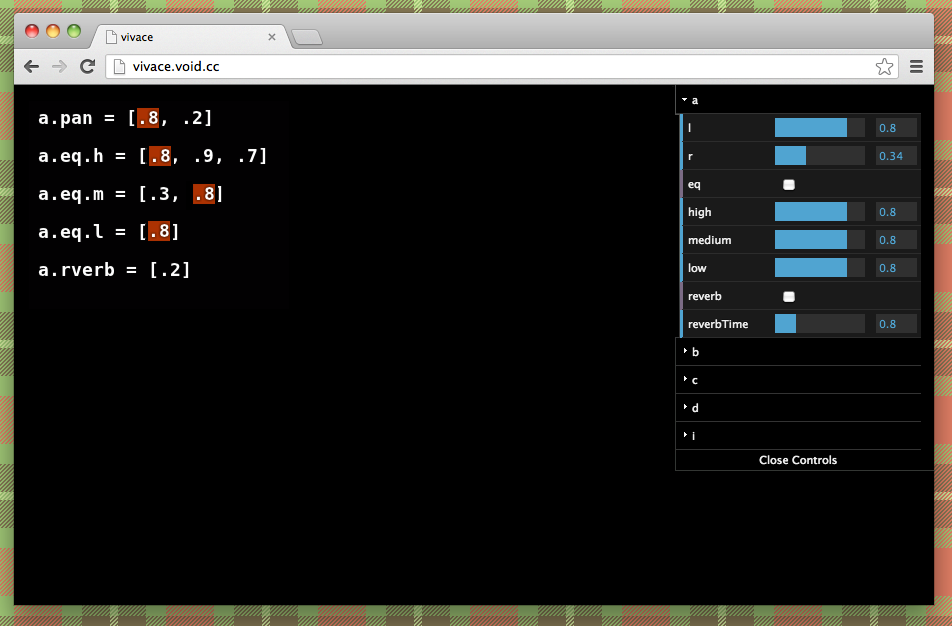
\includegraphics[scale=.3]{img/fig_ui.png}
    \caption{Every audio unit parameter can be manipulated by code or
      using the UI.}
    \label{fig:ui}
  \end{center}
\end{figure}

Vivace supports every audio unit implemented by Web Audio API. It is
possible to load audio files or synthesize in real time using
wave-table oscillators. The default audio chain of each voice can be
modified at any time while it is running. It is interesting to note
the presence of an ``Analyzer'' inside the default chain. It uses FFT
(natively implemented) to expose energies and frequencies, enabling
the use of those values to animate videos and render graphical forms
inside Vivace.

Along with audio, Vivace supports video files. It is possible to
upload files or use YouTube URLs. Videos are treated the same way as
buffer sources or oscillators, i.e.\ as voices, and can be manipulated
on real time, making Vivace a live cinema or a VJing tool.

\section{Into the wild: the raise of freak coding makes it collaborative}

Vivace as a tool enables interaction while everyone could use its own
creativity. The interaction is not mediated by a common score, but by
a mutual desire to create a composition in real time. In this context
born the \emph{freak coder} (Figure~\ref{fig:freakcoder}): someone
that adds up his individuality to others aiming to transform the
computer in an instrument of artistic fruition without restricting to
itself the control of the machine but inviting everyone to join him in
the same activity. A freak coder decides what he is going to do and
amplifies his own comprehension of the computer capacity as an
instrument. By using simple rules, Vivace enables the emergence of the
performance and makes it a kind of a collective game, where the rules,
being visible to everyone, eases audience and specialists alike to
join in.

\begin{figure}[htpb]
  \begin{center}
    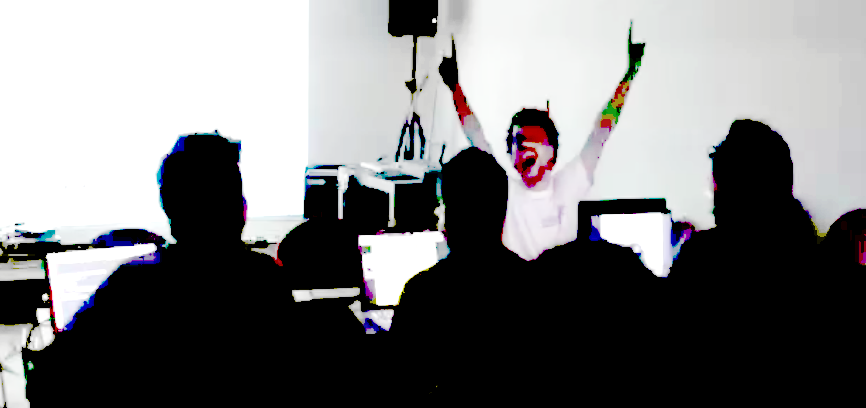
\includegraphics[scale=.4]{img/fig_freakcoder.png}
    \caption{Freak coder: a live coder who, together with others, uses
      popular and freak media to gain audience attention to the shared
      code.}
    \label{fig:freakcoder}
  \end{center}
\end{figure}

Live coding becomes a natural path to the type of use and
technological development in which freak coders are involved, in
confluence with the understanding that technology should never be
treated as a dogma or kept in secret. Live coding is seen as a
behavioral desalination of a digital artist. Not only the code is
displayed and manipulated, but the computer screen and potentially any
interaction between the performance and the computer. The triad
performer, code and audience characterizes the performance as live
coding.  This comprehension was possible after a presentation by
LabMacambira.sourceforge.net at the 9th edition of AVAV
(\textit{\'{A}udioVisual Ao Vivo} or Live Audiovisual), an event where
artists who are experimenting audio and video in real time comes
together to show their works. In this presentation, the authors, Caleb
Luporini and Gera Rocha started without Renato Fabbri and Vilson
Vieira, as they were on their way to the presentation, traveling from
another city. Upon arrival, they both turned their laptops on and
started taking part on the performance in such a way that no
embarrassment or rupture was brought into the happening.  It is
important to state that no previous rehearsal had taken place between
Mr. Luporini and Mr. Rocha~\footnote{Videos were selected beforehand
  by Mr. Luporini alone without knowledge of the other
  performers.}. In the 30 minutes performance, the audience started to
take guidance from messages given on the performance big screen and
edited Vivace code that was being played together with the starting
four performers.

Another artifact noted on this presentation was the emergence, in a
formal environment~\footnote{The four performers were in a light-less
  room, three of them facing the big screen and the other one facing
  the public.}, of a collective euphoria fertilized by a man-machine
interaction. It is the performer posture that takes a spectator to an
experience of a non-spectator and to take part on a highly
technological activity as something playful and possible to be
assimilated.  During the whole presentation, all
labMacambira.sourceforge.net members were smiling and established a
relation of lightness and brotherhood with the audience,
i.e.\ spectators were being constantly invited by the posture of
labMacambira.sourceforge.net members to interact with what was being
proposed.  This exchange between the four elements therein presents --
performers, computer, Vivace and audience -- was able to create an
environment of collaboration and liberty as generators of playfulness
and knowledge unheard of, at least in Brazilian live coding
terms. This is the ``facilitator'' that emerged and received the name
\emph{freak coder}.

To gain attention of the audience, we as freak coders used popular
media as material. The code was shown in front of scenes from
Brazilian novels (as in Figure~\ref{fig:novela}) and B-movies, what
resulted in a freak style, with images of monsters and funny dialogs
between novel actors. In other performances for heterogeneous
attendees the effect was the same as the first presentation where we
used those kind of pop-art: the people was fascinated by the adherence
between the code and the media they see every day on their TV
set. Since that, the use of popular and freak media becomes a
signature of freak coding.

\begin{figure}[htpb]
  \begin{center}
    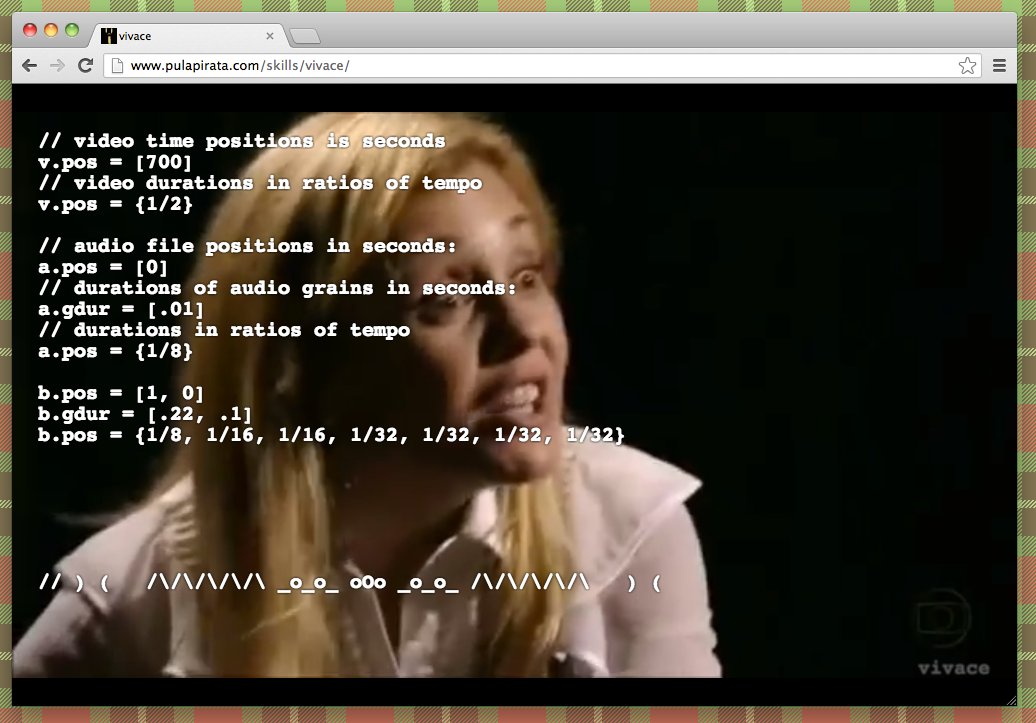
\includegraphics[scale=.3]{img/fig_novela.png}
    \caption{Videos from popular Brazilian novels and B-movies were
      used as material: extreme pop-art as artifice to attract
      audience attention to the code.}
    \label{fig:novela}
  \end{center}
\end{figure}

All labMacambira.sourceforge.net members participates in the Brazilian
free software movement. In this way, freak coding origins should be
looked for inside this movement, a figure raised from the
characteristics presented on Vivace. It is inherent to the free
software movement the continued transmission of what is known. The
same happens on the demystification of technology and the festive and
gregarious behavior. At the performer-computer relation is where this
behavior becomes concrete. More than the materials used in the live
coding sessions, the performer instance in relation to the computer --
as already expressed in the described presentation -- is what really
subverts not just the computer use but the relationship between the
man and the machine. Namely a kind of a ``rock and roll'' stance. The
freak coder breaks, by his own nature, with the stigma of the computer
as the source of a serious and professional posture. In the same way,
breaks with the posture of the scholar performer, stern and closed in
itself. The freak coding is ``rock and roll''. The freak coder becomes
Jerry Lee of technology making ``techno-pyrophagy''. He codes and
smiles at same time. The freak coder seduces through the computer
screen and by the way he codes.

\section{Conclusions and future work}

Vivace was motivated by performances realized in the recently emerging
Brazilian live coding scene. Vivace development was guided by this
direct contact of performers and the public. The language was designed
and implemented after the identification of common patterns already
used on presentations. Following a open source practice, Vivace is
being developed by many hands from computer scientists, musicians,
activists and social scientists. The language is not perfect at all,
but is growing as a balance between flexibility and restriction,
making it an interesting language to artistic expression on
collaborative sessions.

It is important to note the advantage of using Web as the platform for
experimentation on live coding and other computer music
developments. The recent APIs like Web Audio together with means to
easily prototype UI and language parsers creates a prolific
scenario. Henceforth the most interesting characteristic is the
collaboration proportioned by Web. Using collaborative editors we can
expose an entire music program to be edited by anyone, anywhere.

Vivace, although a ``freak coding'' language, is constrained in its
music expression. Having a domain specific language as Vivace is
interesting to express some musical ideas while others became hard or
even impossible to be expressed. In this context we assume Vivace as a
first step to create other languages and collaborative systems,
emerging from live coding practices. In this way, we can tell that
those performances and even Vivace are motivating the creation of
other live coding tools. Carnaval~\footnote{Carnaval is being
  conceived as free software and a collaborative art piece since its
  beginning. The first sketches are on-line at
  \url{http://pontaopad.me/vj}} is one of these new realizations, it
can be seen as a ``personal TV channel''. Each channel has a Vivace
instance running on it, making possible for anyone to remix media and
create their own composition. It is a social network of live coded
remixes. Vivace, instead of an isolated piece of software is then used
as a module, part of Carnaval.

In our experiences as performances and developers of live coding
languages we can assert this style of music realization as
inspirational and flexible. Nevertheless, we continue to search for
improvements on Vivace -- and others derived tools -- to increase the
already consolidated objective of live coding as a musical practice:
turn the computer music performance more human, more interactive with
audience.

Future improvements are planned on Vivace: the possibility to
explicitly define large music arcs as nested sequences related to
audio units, the use of 3D graphics APIs to render forms -- passive to
be changed by currently running audio parameters -- and text messages
to the audience, and improved UI to make the code editing more
flexible and reactive~\citep*{brett}.  Along with the language and
system itself, this paper is a live initiative. The freak coding as an
artistic style will be explored more deeply on future studies --
regarding its own aesthetics -- and in already planned performances.

We want to end underlining the social importance regarding live
coding. The authors, although working on the same collective, were not
working close to each other since the creation of Vivace and the rise
of freak coding. The performances were provided by the union of those
artists. Their union created their own tools and influenced their own
attitude. And the circle starts again.

\bibliographystyle{cmj}
\bibliography{cmjbib}
\end{document}
